\chapter{Deep Learning}

Deep Learning (DL) is a subfield of Neural Networks (NN) which in turn is a subfield of Machine Learning (ML) which again is a subfield of Artificial Intelligence (AI). Figure \ref{fig:MLOverview} shows a Neural Network relevant taxonomy of AI. There are many advantages of ML over more traditional statistical methods as often found in statistical learning. Some of them are that ML does not require any hypothesis and deep understanding of the underlying data. While statistical learning is mostly about inference (deducing properties of an underlying probability distribution, sampled from a larger population), ML is mostly about predictions in supervised, unsupervised and semi-supervised learning. It also does not operate on assumptions like normality, multicollinearity and homoscedasticity etc.. Statistical Learning operates on much smaller datasets with only a few attributes and therefore is less fit for problems with millions of possible and possibly unknown attributes and data samples. Machine Learning excels at identifying patterns from large datsets through iterations and being able to predict or classify previously unseen data.
Traditional Machine Learning approaches were based on very specific feature extractions that needed to be found/created manually and could take months to fine tune. The biggest downside was that the features often were not generalizable but were very domain specific. Even looking at the same object from different angles or from different photographs often needed additional fine tuning of existing features or creating new ones. Some of the feature extraction algorithms include Scale Invariant Feature Transform (SIFT), Histogram Oriented Gradient (HOG), Local Binary Pattern (LBP). Learning algorithms that are applied on these features are e.g.: Support Vector Machines (SVM), Random Forest (RF), Principal Component Analysis (PCA), Kernel PCA (KPCA), Linear Decrement Analysis (LDA), Fisher Decrement Analysis (FDA) and many more \ref{fig:MLOverview}. New Machine Learning methods are able to automatically learn feature representations which is much less labor intensive and often very surprising as features are learned that don't intuitively make sense [TODO: show some examples] but perform really well, but sometimes things are learned that correlate with the provided labels but have no causality [TODO: some counter examples].

\begin{figure}[H]
  \centering
  \caption{Partial taxonomy of Artificial Inteligence \cite{alom2018history}}
  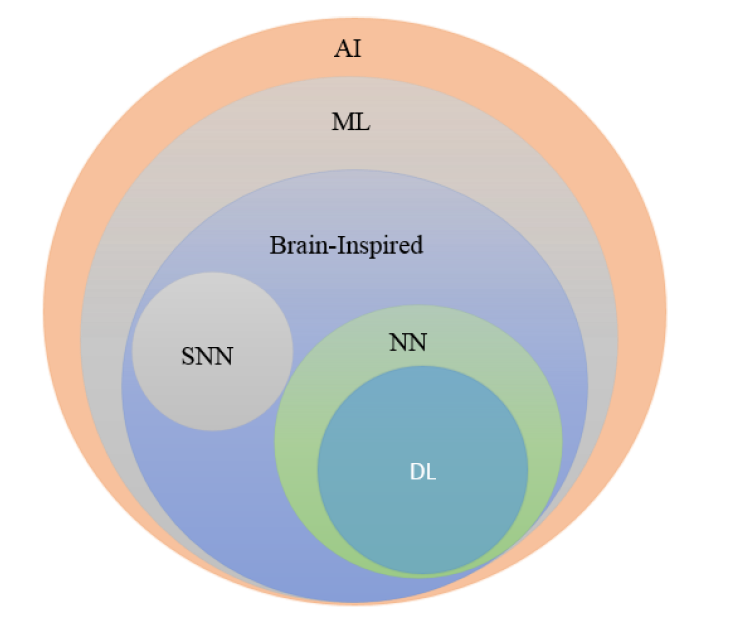
\includegraphics[scale=0.4]{chapter3/MLOverview}
  \label{fig:MLOverview}
\end{figure}

An Artificial Neural Network (ANN) tries to mimic the behavior of the human brain to a primitive extent. The analogy of the artificial neuron helps to understand the parallels between how biological neurons pass information but it is only an analogy and therefore should be used very cautiously. There are more differences than similarities and the human brain is still in many aspects a mystery to be solved. Nonetheless the abstract notion of a neuron is visually very appealing and useful. Figure \ref{fig:Neurons} show on the left side a biological neuron with all its relevant parts and the mathematical representation of it on the right side. The biological neuron receives its inputs from other neurons through its dendrites (through many different neurotransmitters in the synapses). If a certain threshold is reached in the cell body from all its dendrites, it transmits the information along the axon to other neurons. The axon branches out at the and reaches several different neurons and the process continues. Learning is believed to happen when the sensitivity of the synapses changes and new pathways are formed through branching the axon and connecting to new axons or making the current pathways stronger.

\begin{figure}[H]
  \centering
  \caption{A biological neuron on the left versus the mathematical representation of neuron how it is used in neural networks on the right. \cite{cs231neuralnetworks}}
  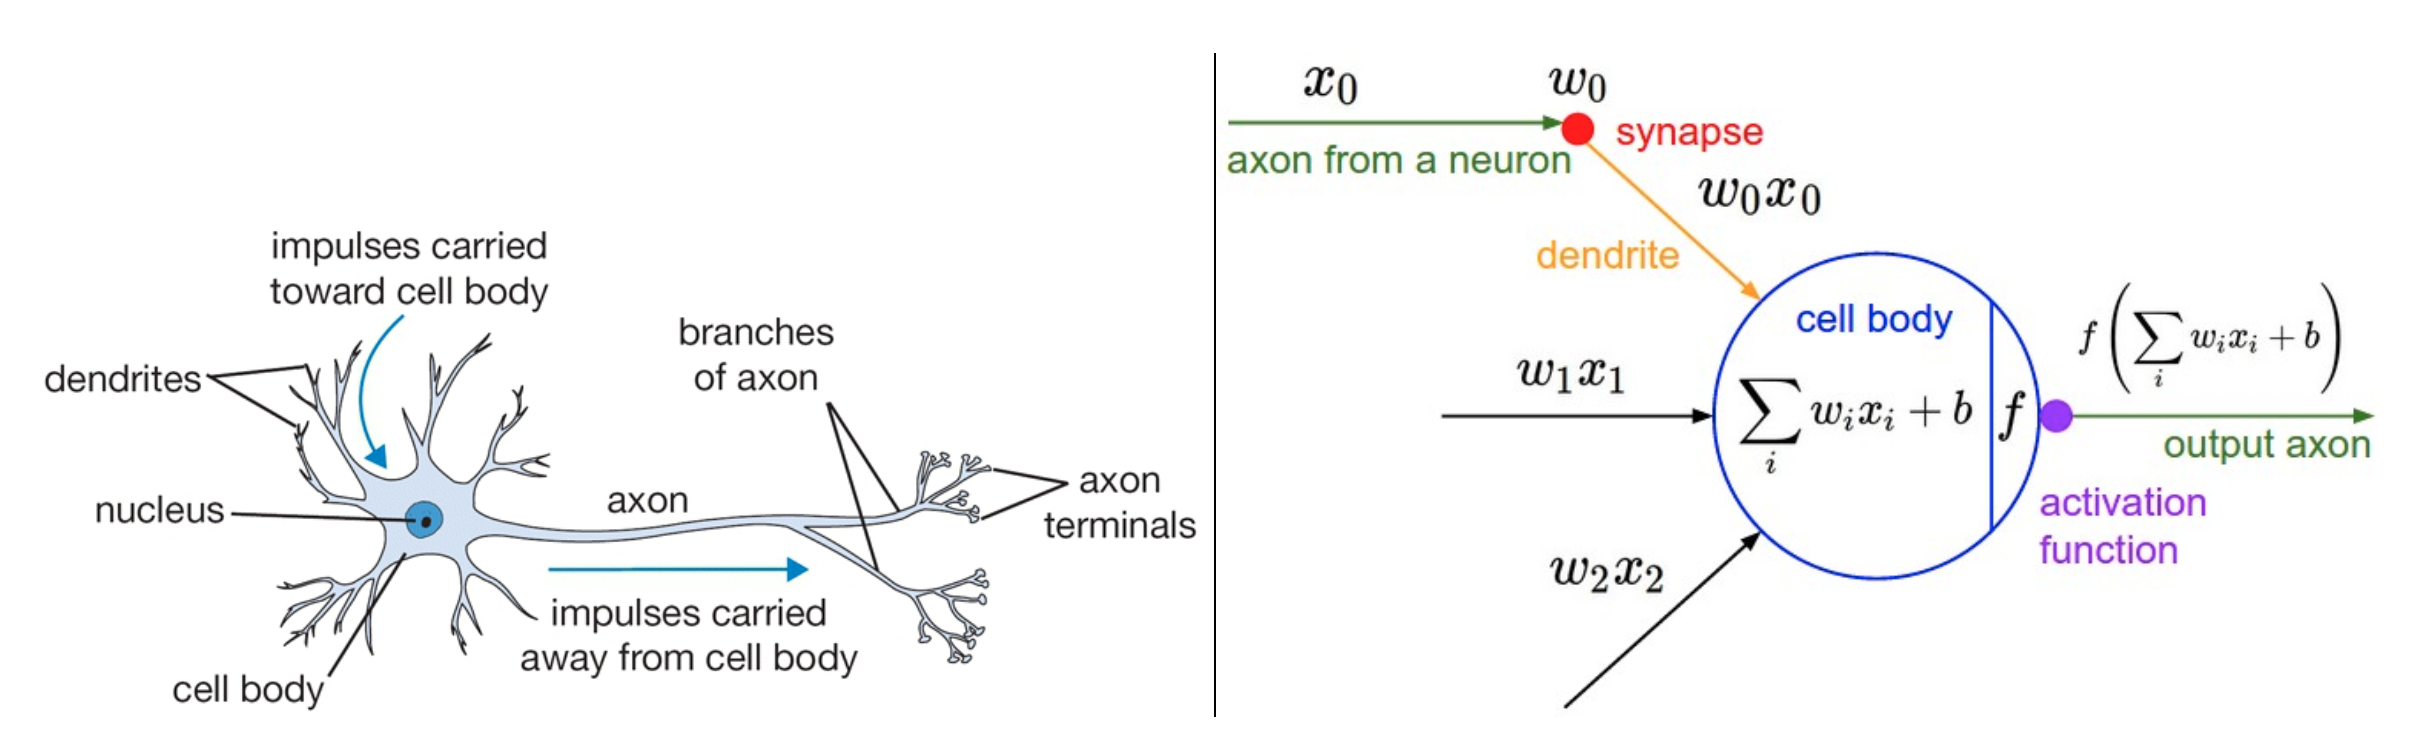
\includegraphics[scale=0.35]{chapter3/Neurons}
  \label{fig:Neurons}
\end{figure}

This is indeed similar to how an artificial neuron processes information and passes it forward. An artificial neuron receives inputs (e.g. $x_0$) from other neurons and applies a weight matrix (e.g. $w_0$) and a bias (e.g. $b$) on it. The weights and biases can be compared to the strength of the synapses in the biological neuron and these can be changed through learning. Actually that's what happens during the backpropagation explained later on. The weights are adjusted in order to classify the input more accurately. In the cell body of the mathematical representation performs a dot product between the inputs and the weights adds the bias ($w_i x_i + b$) and then applies some kind of activation function. This activation function needs to be non-linear, because otherwise all the matrix computations of different neurons could be collapsed into one linear computation and no learning would take place. Just a linear regression would be achieved.
Traditionally a sigmoid function has been used for the activation function since it takes any real number as inputs and outputs numbers between 0 and 1. That is a very intuitive non-linearity function to work with but has some disadvantages when backpropagating the loss function and adjusting the parameters in the weight matrices.  During backpropagation the loss is computed according to some loss function and then back propagated through all layers and units. During that process the partial derivatives of the loss function are computed with respect to the input variables (e.g. $x_i^j$) of that specific unit. In the used notation the superscript denotes the layer whereas the subscript denotes the unit. These derivatives are then multiplied by a learning rate alpha and added to the current weights. This process of changing the weights towards a optimal loss is called learning and happens through many iterations. In Figure \ref{fig:SigmoidTanh} the two activation functions, the sigmoid and the tanh, are shown. Since the partial derivatives are crucial in learning - the stepper the derivation the bigger the change in weights - the disadvantages of both non-linearties are clearly visible towards the borders. If the function moves mostly horizontally, the first derivation will be near 0 thus learning happens very slow. The tanh has a much steeper function around the center (leading to a bigger first derivative) but still has the same problem towards the borders.

\begin{figure}[H]
  \centering
  \caption{The sigmoid non-linearity takes in any real number and outputs a number in the range [0,1], wheras the tanh non-linearity takes the same input but outputs a number in the range of [-1,1]. \cite{cs231neuralnetworks}}
  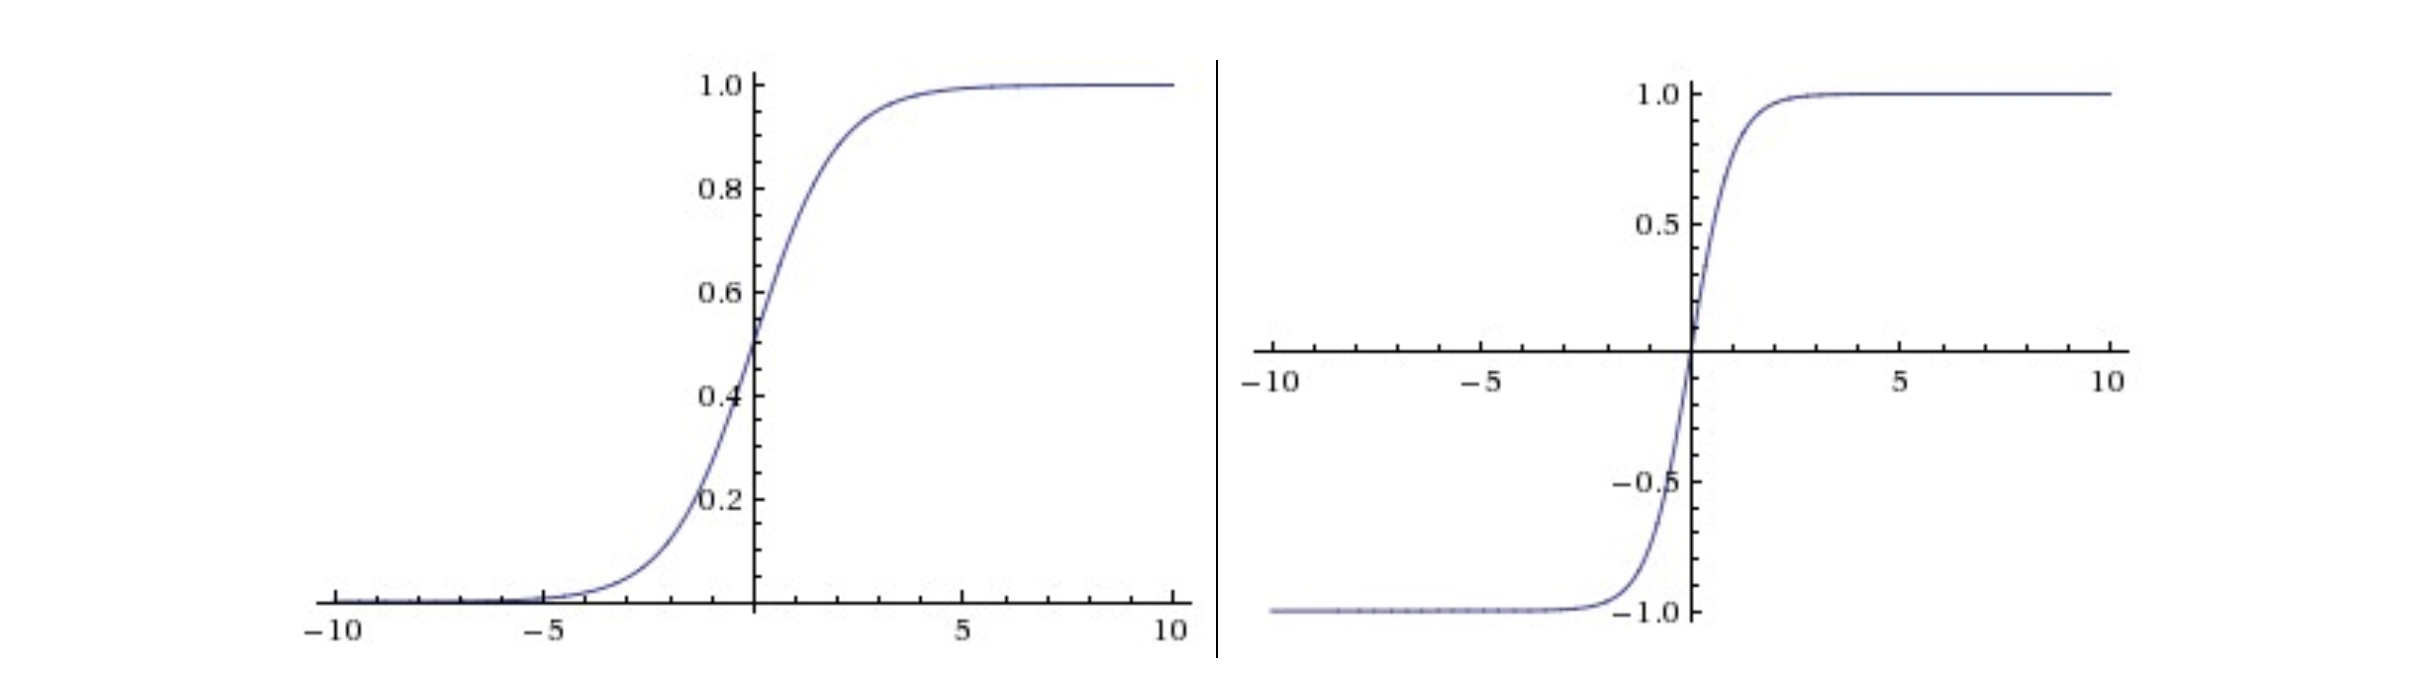
\includegraphics[scale=0.35]{chapter3/SigmoidTanh}
  \label{fig:SigmoidTanh}
\end{figure}

For the above mentioned reasons, the sigmoid non-linearity is not used anymore except in the last layer and only if the task is a binary classification. For that special case the sigmoid is still a valid function. As an alternative the Rectified Linear Unit (ReLU) is used. It is very simple, fast to compute and easy to back-propagate since the derivatives are 0 or a fixed value. In order to omit the deactivation of units, which happens if the input values are smaller than 0, a leaky ReLU can be used. Both non-linearities can be seen in Figure \ref{fig:ReLU}.

\begin{figure}[H]
  \centering
  \caption{Rectified Liner Unit on the right side. Deactivating units if their input values are negative. Leaky ReLU that never deactivates units. \cite{reinventingNN}}
  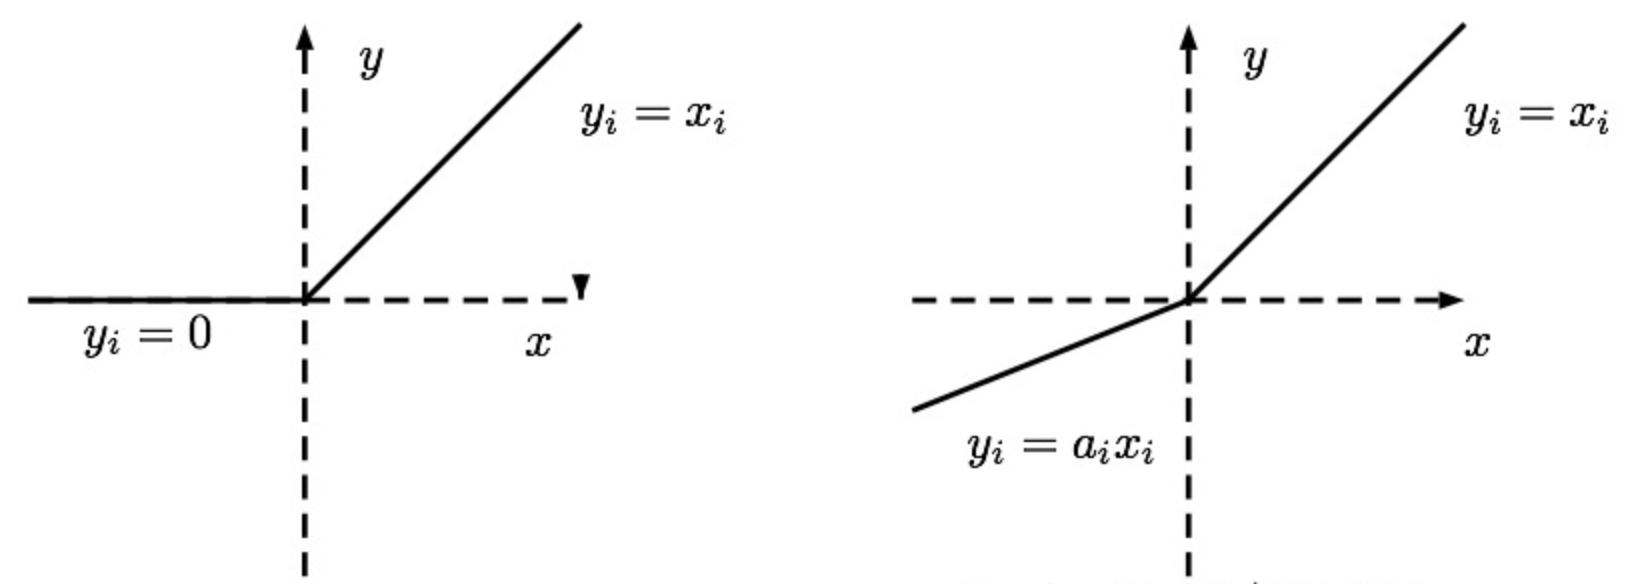
\includegraphics[scale=0.35]{chapter3/ReLU}
  \label{fig:ReLU}
\end{figure}

The components of an Artificial Neural Network (ANN) are the units (neurons) organized in an acyclic graph. All units that are reached from the input layer by the same amount of hops are organized into layers. These units are not connected to each other but to next layer as shown in Figure \ref{fig:MLP}. As the name suggests cycles are not allowed since the forward and backward pass would not be well defined anymore. Another big difference to the human brain where acyclic connections are possible and very common [TODO: find relevant reference]. Subsequent layers within the ANN are most commonly fully connected with each other, meaning every unit connects to every unit in the next layer. These networks are also often called Multi-Layer Perceptrons (MLP). One of the problems with MLP's is that the fully-connected nature of this architecture increases the number of parameters exponentially. E.g. an RGB image of 256 by 256 pixels as an input size of 196'608 (256x256x3). If this is multiplied with the next layer having 1000 hidden units the result is already 196'608'000 meaning there are roughly 197 million parameters to be held in memory and updated with every iteration just for the first layer. Every unit in this layer would have 196'608 weights which is wasteful since so many parameters with rather simple images lead to severe overfitting. Another big disadvantage for image recognition is the fact that there is no spatial encoding in the network. Is is very nicely observed with the MNIST dataset where images (28x28 pixels) of handwritten digits are provided \cite{MNISTdatabase}. The MLP learns that the image contains a certain number only by learning which pixels need to be black in order to match the previously seen labels. That leads to a near perfect recognition of the centered digit 2 but if the digit is moved to the border (different distribution of black pixels) the MLP is not able to recognize the digit anymore.

\begin{figure}[H]
  \centering
  \caption{. \cite{cs231nconvolution}}
  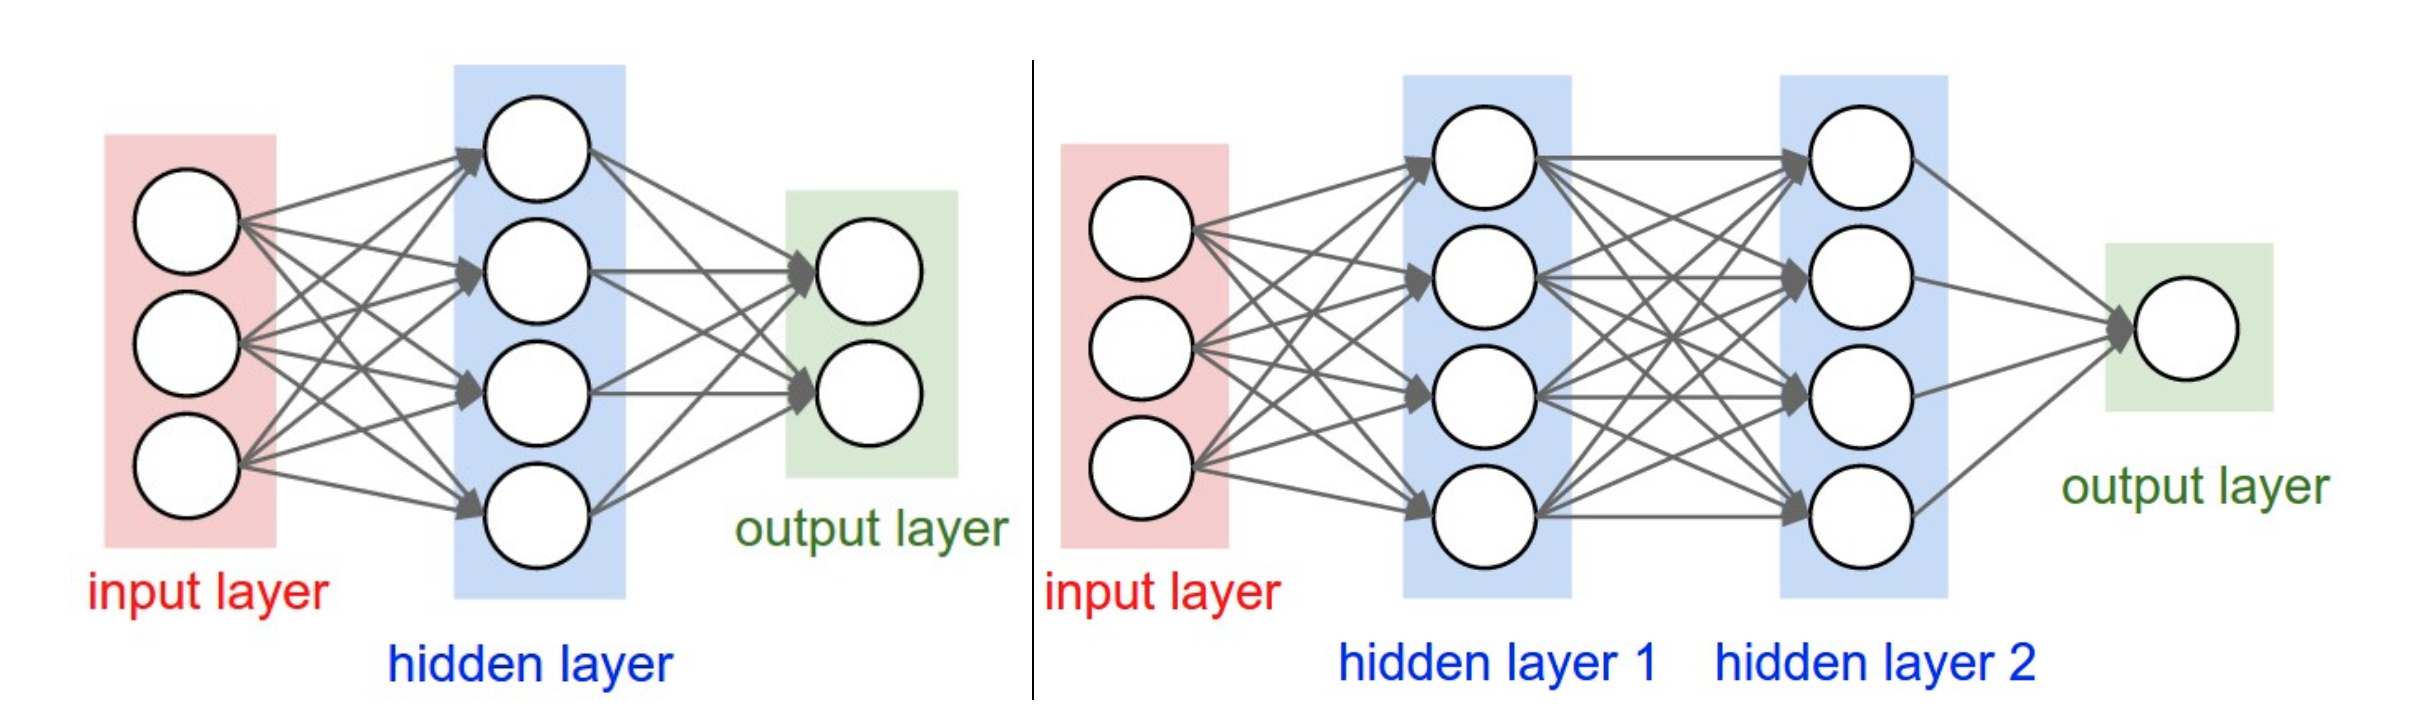
\includegraphics[scale=0.36]{chapter3/MLP}
  \label{fig:MLP}
\end{figure}

\section{CNN}

Convolutional Neural Networks (CNN) are a subset of Neural Networks so they still share most of the components like an input layer, hidden layers with its units, fully connected layers at the end of the architecture, a loss function, forward and backward propagation. The big difference is that CNN's explicitly expect images as input whereas a Neural Network expects nothing in particular, just a single vector. Knowing that the input is an image, the architecture can be changed accordingly, leading to spatial awareness through convolutions and vastly reduced parameters. Spatial awareness means that additionally to knowing the value of one pixel (in the first layer) a convolution encodes the values of neighboring pixels, thus giving some representation of an area of nearby pixels. Figure \ref{fig:Convolution} shows a simple convolution step where a filter of 5x5x3 is layed over the image. The filters depth (3rd dimension) is always equal to the input volumes dimension. Since the image is RGB encoded the dept of the image is 3, so are the filter in the first layer. The filter, sometimes also called kernel, is then convolved across the whole image and computes a dot product at every position. This gives an activation map, seen in blue on the right side in Figure \ref{fig:Convolution}. Each filter that is convolved across the image produces a different activation map that usually is slightly smaller than the original input but becomes deeper with every additional layer, since more filters are added. The goal of the learning process is to learn filter, that represent specific characteristics of the image and help in correct classification (reducing the loss). As mentioned in the beginning of the chapter, a huge advantage of modern machine learning methods is that the feature maps are learnt automatically by the model. The best filters will get found without the need of manually crafting specific HOG features. That saves time and leads to much more generalizable models.

\begin{figure}[H]
  \centering
  \caption{. \cite{cs231nconvolution}}
  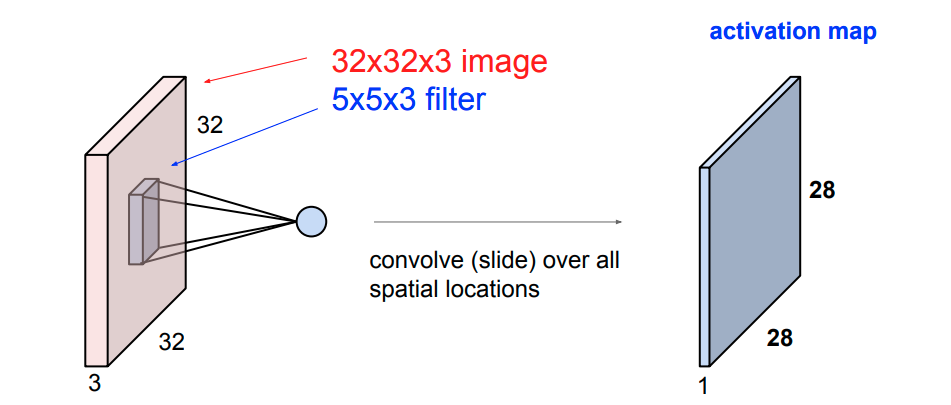
\includegraphics[scale=0.35]{chapter3/Convolution}
  \label{fig:Convolution}
\end{figure}

Instead of connecting all the neurons of one layer to all the neurons of the subsequent layer leading to an exponential growth of parameters, now each neuron is only connected to a local region of the input. The 5x5x3 filter shown in Figure \ref{fig:Convolution} has receptive filed of 5x5. The depth of the filter must always be equal to the depth of the input volume (input image in the first layer).

In order to build a CNN three main components are used. The convolution layer which is described above often followed by a Pooling Layer that reduces the width and height, while keeping the depth as is. In the end the third component is a Fully Connected Layer. Often the Fully-Connected Layer also consists of a softmax function that gives the probability of the image being one of each classes. Between the Convolution Layer and the Pooling Layer the activation function (e.g. ReLU) applies elementwise. The activation function does not change the dimensions but simply squashes the values into the range of [0,x] in case of a ReLU. A typical Convolutional Network would have the following architecture [INPUT - x * (CONV - RELU - POOL) - FC]. The higher the variable x the deeper the CNN.

The Pooling Layer's goal is to reduce the width and height of the input volume without reducing its depth. That leads to less parameters in the network and less overfitting. The architecture needs to focus on the relevant parts of the image instead of trying to optimize too many parameters and thus overfit to already seen images. Pooling Layers mostly apply the MAX function and are of size 2x2. The MAX function is computationally very cheap and the size of 2x2 let's the volume half in width and height. The highest value in the 2x2 mask is kept. Figure \ref{fig:MaxPooling} shows the MAX-Pooling process.

\begin{figure}[H]
  \centering
  \caption{. \cite{cs231convnetworks}}
  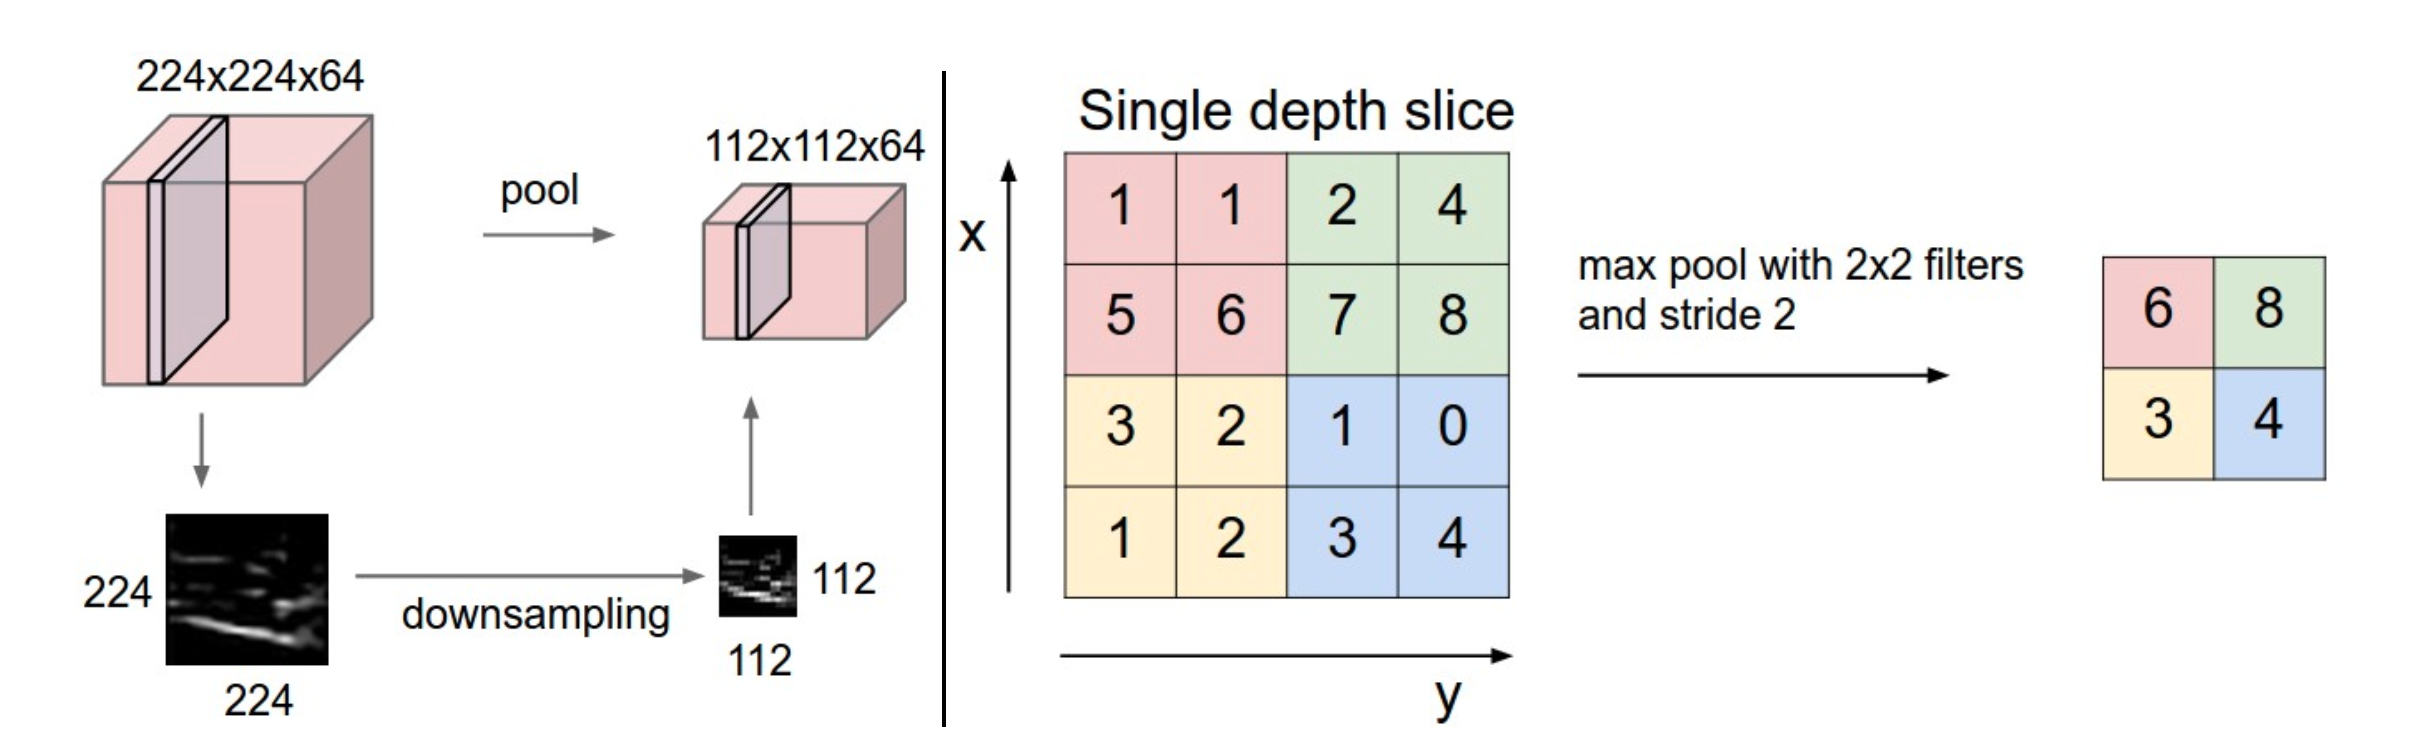
\includegraphics[scale=0.35]{chapter3/MaxPooling}
  \label{fig:MaxPooling}
\end{figure}


\section{ImageNet Large Scale Visual Recognition Challenge (ILSVRC)}

The ImageNet Large Scale Visual Recognition Challenge (ILSVRC) has become the standard benchmark for object recognition and is held anually since 2010 \cite{imagenet}. It has borrowed many concepts from the PASCAL VOC 2010 dataset but increased the amount of data drastically, from 19'737 images in PASCAL VOC 2010 with 20 object classes to 1'461'406 images and 1000 object classes in ILSVRC 2010 \cite{everingham2010pascal, russakovsky2015imagenet}. ILSVRC consists of two components: the dataset that is publicly available and consists of over 1.2 million annotated, high-resolution images (train set), and the annual competition with its workshops. The test set, ranging from 100'000 to 150'000 images, is also released but without the labels. Participants are able to train their models on the datasets and annotate the images in the test set. The annotated test set is then send to the evaluation server where the overall score is computed \cite{russakovsky2015imagenet}. With the ImageNet Challenge there are two main competitions namely object detection for 200 fully labeled categories and object localization for 1000 categories (binary label for presence or absence of an object). For the object localization there are two main metrics, the top-1 error rate and the top-5 error rate. The top-1 error rate shows the percentage for which the correct class was failed to be correctly predicted (only the first top label is observed). The top-5 error rate shows the percentag of test examples for which the correct label was not in the top 5 predicted classes. Since ILSVRC 2015 new competition tasks are added like object detection from video or scene classificiation, but they are less relevant for this thesis \cite{imagenet2015}. Before ILSVRC many datasets were available for training models like Caltech 101 \cite{fei2007learning} with 101 object classes and Caltech 256 \cite{griffin2007caltech} with 256 object classes. Both were tiny at best when compared to the ImageNet dataset. TinyImages \cite{torralba200880} is huge with its 80 million images but the images are only 32 by 32 pixels which makes them low-resolution and not manually verified thus leading to many incorrect labels.

In 2010 and 2011 the winners used traditional machine learning approaches like HOG, LBP and FV for dense grid descriptors and SVM for feature application with other more specialized methods. In 2012 AlexNet, a 5-layer CNN, beat all competitor by a large margin. It was the beginning of a new chapter in machine learning namely the chapter of Convolutional Neural Networks and Deep Learning in the field of computer vision. Since then, only CNN's are winning the ILSVRC with ResNet surpassing human level accuracy in 2015 \cite{he2016deep}. Human level accuracy was obtained when Andrej Karpathy took it on and labeled 1'500 test images after having trained on 500 validation images. It took him a few days and he reached an astonishing 5.1\% top-5 error rate while other scientists giving it a try reached around 12\% error rate \cite{humanlevel2014}.

It is also worth noting that ImageNet is the most widely used dataset for transfer learning. Pre-trained weights for most of the current state-of-the-art architectures are widely available on the internet and can be downloaded. All evaluation in Chapter 5 related to transfer learning is based on weights pre-trained on ImageNet.

\section{AlexNet}

In 2012, a paper by Alex Krizhevsky started the new era of Convolutional Neural Networks, where CNN's were not only practibly applicable to current visual problems like the ImageNet Large Scale Visual Recognition Challenge (ILSVRC), but beat the best results by a big margin \cite{krizhevsky2012imagenet, imagenet}. The architecture by Alex Krizhevsky, a 5-layer CNN, achieved 15.3\% top-5 error rate, and was named AlexNet after its creator. The next best result achieved a top-5 error rate of 26.2\% with versions of Fisher Vectors (FV) and Graphical Gaussian Vectors (GGV) after going through a feature extraction process with SIFT, CSIFT, LBP and GIST. Since then the winners of all subsequent ILSVRC challenges apply all successfully a deep learning approach. \\

AlexNet uses eight learned layers of which five are convolutional, and three are fully-connected layers. After the convolutions, ReLU's are used for the activation function since they train several times faster than equivalent architectures trained with tanh or sigmoid functions. The last fully-connected layer is fed to a 1000-way softmax function that produces a distribution over all the 1000 classes giving the probability of a certain class to be contained in the image. For the input layer the images are first resized to 256 by 256 pixels and then crops of size 227 by 227 by 3 are used as inputs into the model. 96 kernels of size 11 by 11 by 3 with a stride of 4 pixels are then applied on the input image leading to a output volume of 55 by 55 by 96. In the original paper the filters were split across two GPU's but since the GPU's have increased their capacity and performance since 2012 hugely, this splitting is not applied on the current model. The formula for calculating the new output volumes is the following: \\

\[ O = {\frac{(W - F + 2P)}{S}} + 1 \] \\

with O standing for the output dimension (length of the width or height), W standing for the input length, F for the filter size, P for padding and S for stride. Maxpooling is done after the first, second and fifth convolutions. Instead of going with the regular 2x2 pooling that halfes the width and length dimensions of the input volume, AlexNet applies a 3x3 pooling with stride 2. They argue that it helps in reducing overfitting and leads to slightly better accuracies. The architecture can be seen in figure \ref{fig:AlexNet}. \\

\begin{figure}[H]
  \centering
  \caption{The original architecture as proposed by Alex Krizhevsky with the distribution of the model and filter over two GPU's. \cite{krizhevsky2012imagenet}}
  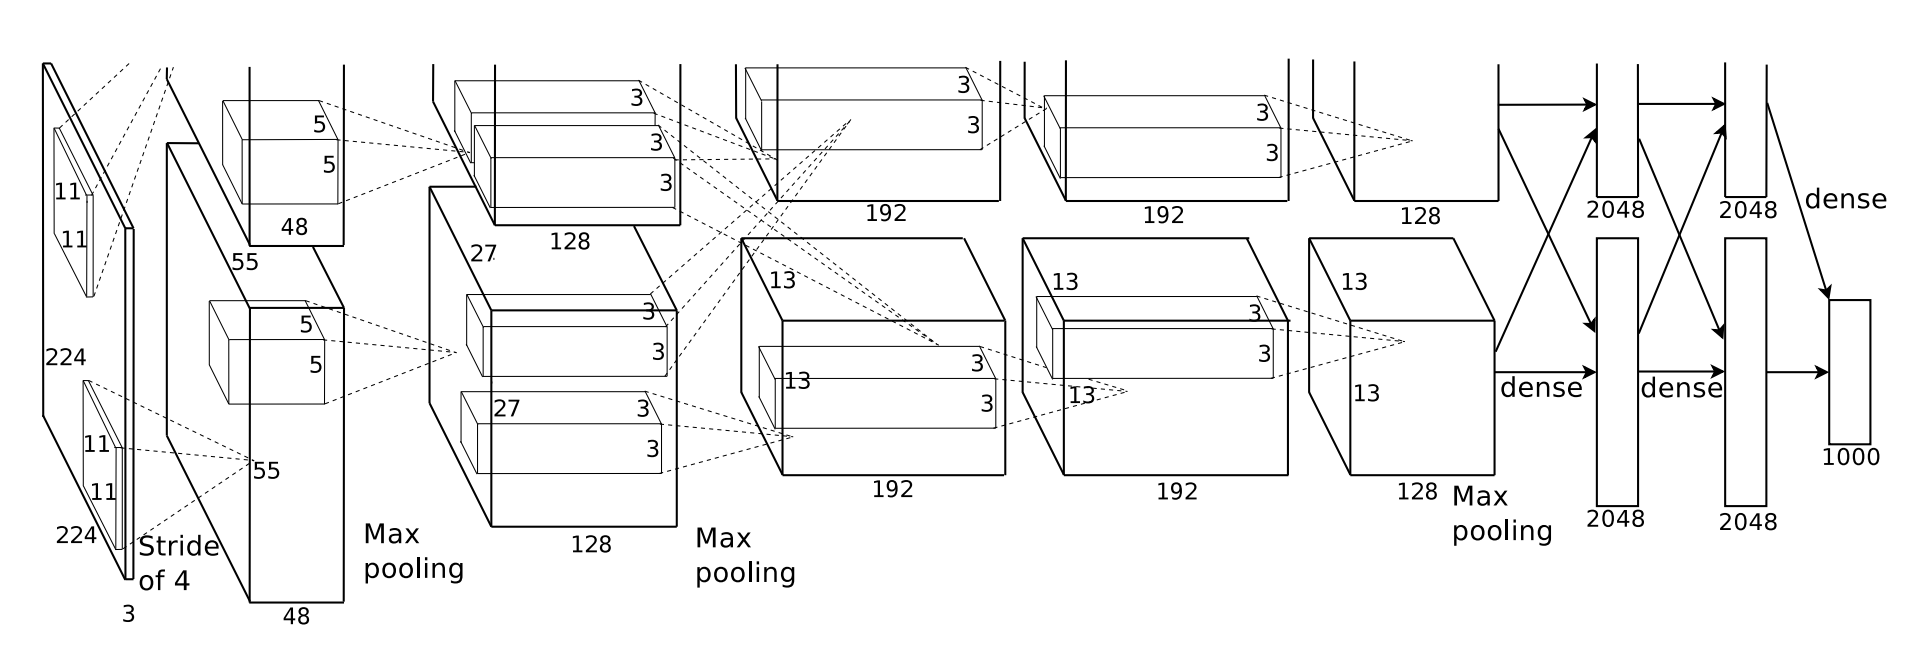
\includegraphics[scale=0.35]{chapter3/AlexNet}
  \label{fig:AlexNet}
\end{figure}

The horizontal seperation of the architecture comes from the need to distribute the model and the filters over two GPU's. Unfortunately the image was already cropped that way in the original paper of Alex Krizhevsky. \\

Although the architecture itself is very small compared to the later architectures, it still has over 60 million parameters to learn. These parameters are mostly located in the first and second fully connected layer. Learning so many parameters for classifying only 1000 objects leads to overfitting to the data trained on. For the ILSVRC competition two methods have been used. Heavy data augmentation using label-preserving transformations (increase images by factor 2048) and dropout in which certain hidden units are dropped for the current forward pass with some probability (often 0.5). \\

The winner of the ILSVRC 2013 was ZFNet which basically is the AlexNet architecture with very small alterations \cite{zeiler2014visualizing}. Although the alterations are small they were very guided in their developement through visualization techniques. Zeiler and Fergus visualized the layers and filters and deduced clear and specific improvements on AlexNet.

Karen Simonyan and Andew Zisserman

\section{VGG}

The 1st runner up winner of the ILSVRC 2014 were Karen Simonyan and Andrew Zisserman with their architecture named VGG \cite{simonyan2014very}. Instead of further trying to fine-tune AlexNet they explicitly wanted to explore how depth of an architecture plays out on accuracy and generalizability. For that reason they used only 3 x 3 convolutions with padding of 1 pixel and stride of 1 pixel as well followed by a ReLU activiation function. Therefore the input volume from layer to layer stays the same while the number of filter increase after each maxpooling layer. If the spatial resolution needs to be reduced, maxpooling is applied with a 2 by 2 windows and stride 2. This allowed Simonyan et al. to push the depth of the network to 16-19 layers. In the end there are again 3 fully-connected layers as in AlexNet. The first two have 4096 hidden units and the third performs a softmax on the 1000 classes of ImageNet dataset. Figure shows the original VGG16 architecture.

\begin{figure}[H]
  \centering
  \caption{VGG16 architecture with 13 convolutional layers and three fully-connected layers at the end. \cite{ferguson2017automatic}}
  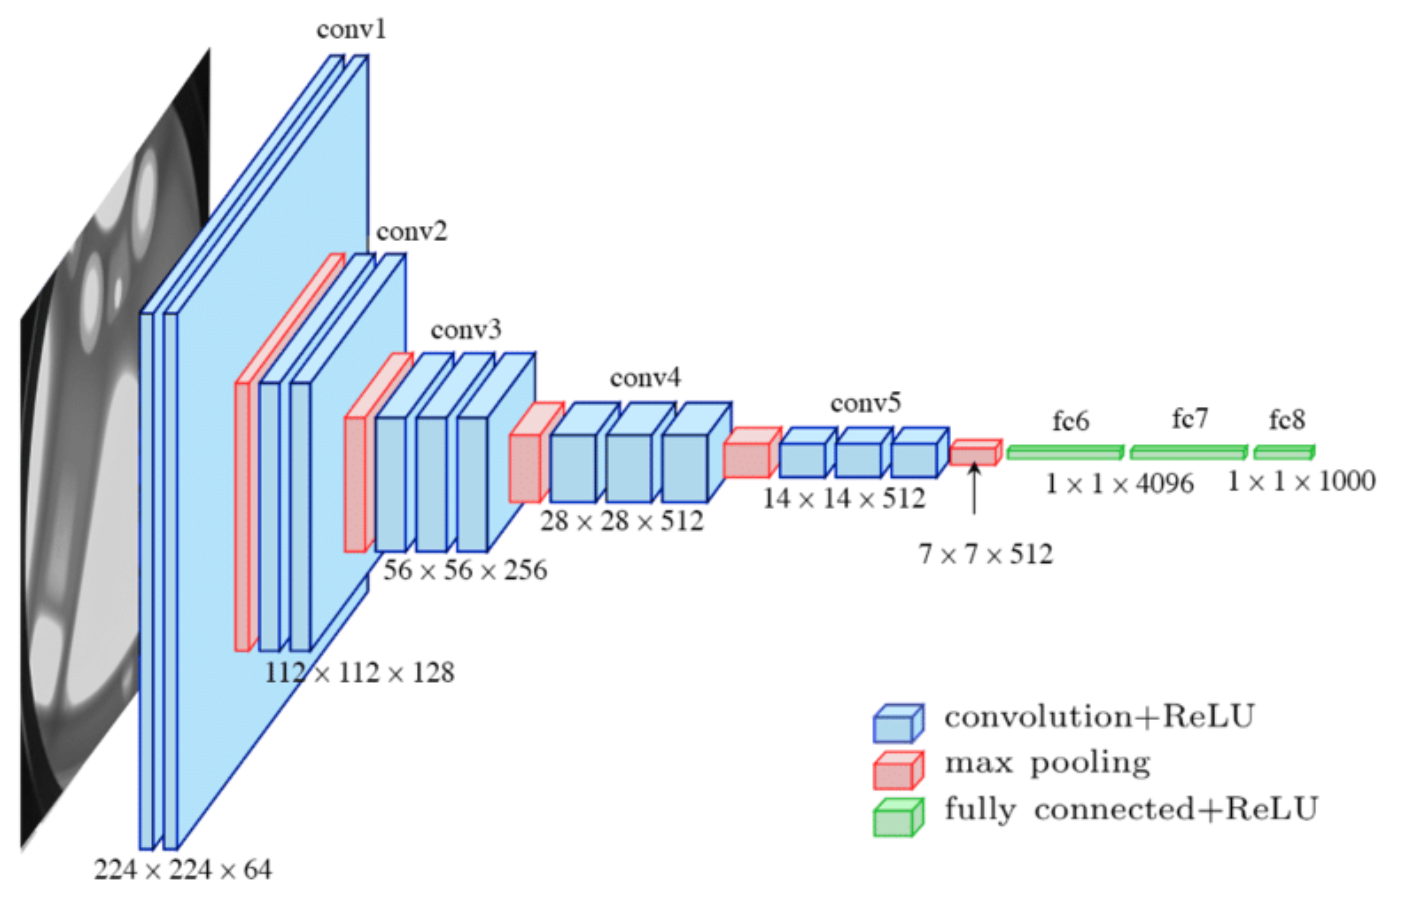
\includegraphics[scale=0.35]{chapter3/VGG16}
  \label{fig:vgg16}
\end{figure}

One of the bigger issues with VGG architectures are their huge size in parameters, which ranges from 133 million parameters for the smaller VGG11 architecture to 144 million parameters for the bigger VGG19. This is problem, since it can be difficult to handle so many parameters and training takes much longer. The last three fully-connected layers contribute the large part of the parameters with the convolutional layers playing a minor role. Because VGG is very uniform with it's 1 type of convolution and easy to understand, it enjoyed large acceptance with the community. Figure \ref{fig:parameters} shows how different architectures perform relative to their size in parameters.

\begin{figure}[H]
  \centering
  \caption{Performance of different architectures relative to their number of operations needed for one forward pass. The number of operations is proportional to the number of parameters used by the architecture. \cite{canziani2016analysis}}
  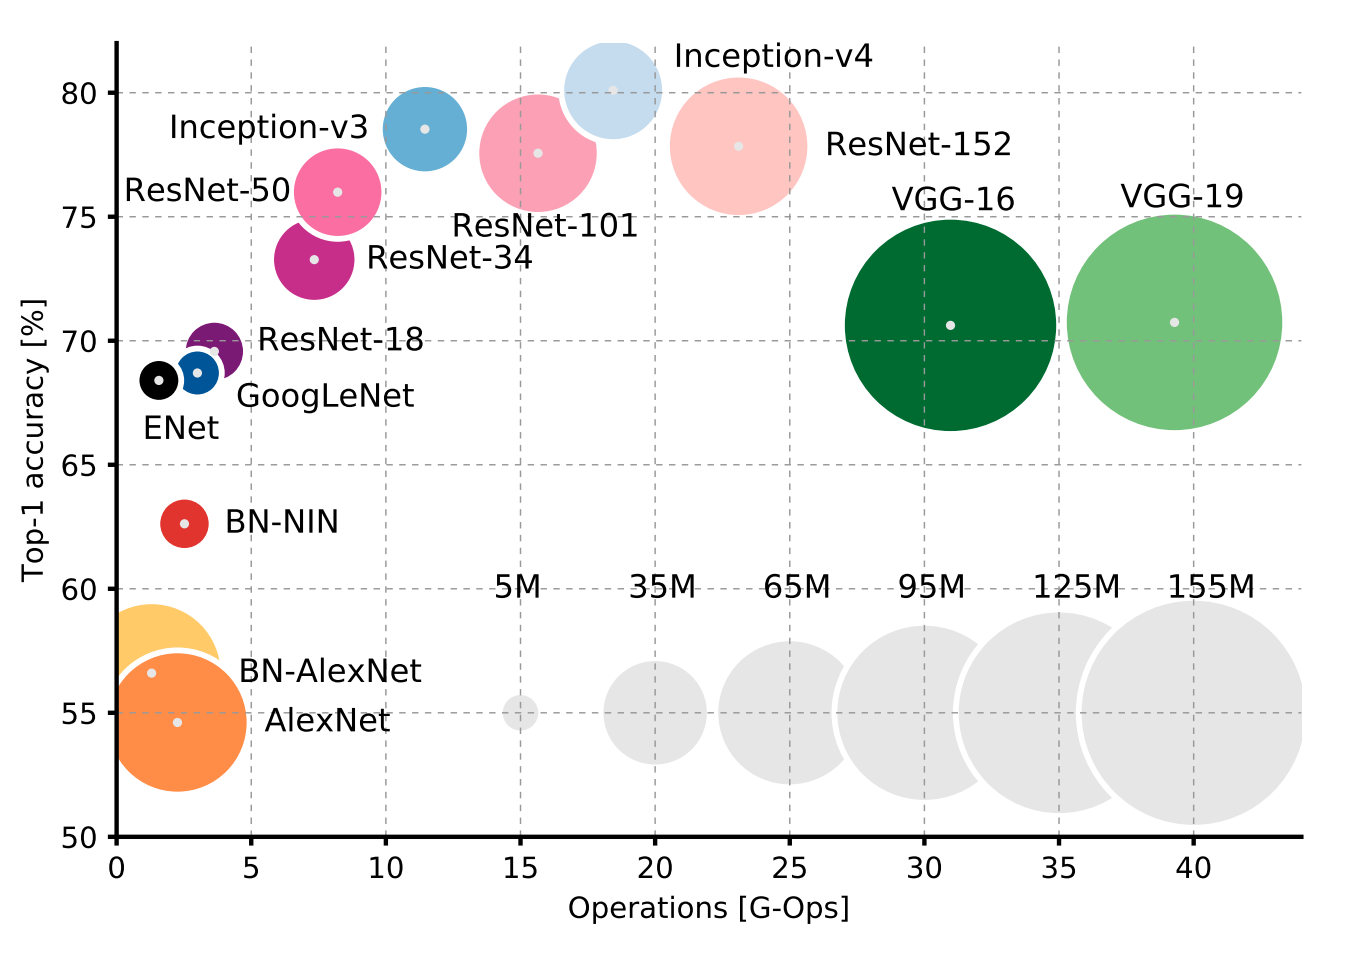
\includegraphics[scale=0.35]{chapter3/parameters}
  \label{fig:parameters}
\end{figure}

\section{Inception}

The winner of the ILSVRC 2014 image classification were Szegedy et al. with their GoogleLeNet architecture \cite{szegedy2015going}. Their network is quite different to the previous networks winning the ILSVRC competitions and applied 1 by 1 convolutions and global average pooling, both methods inspired from the Network in Network paper \cite{lin2013network}. Another technique added to the architecture is the inception module, which has convolutions of different sizes for the the same input volume and stacking the results all into an output volume. \\

The 1 by 1 convolution is used to reduce the dimension along the length axis. E.g. in VGG with every max pooling layer the spatial dimensions got reduced by half but the length of the volume gets deeper with every additional max pooling layer, adding more filters to the computation. With a 1 by 1 convolution the spatial dimensions are untouched but the length will be recast into the the length of number of filters. Also the computational effort gets reduced drastically with this method. In Figure \ref{fig:InceptionRegularConv} a regular 5 by 5 convolution is performed on the input volume of 14x14x480 with 48 filter leading to an output volume of 14x14x48. Computationally that is very expensive with roughly 113 million single operations ( (14x14x48) x (5x5x480) = 9'408 x 12'000 = 112'896'000 ).

\begin{figure}[H]
  \centering
  \caption{5 by 5 convolution is used with only 48 filters reducing the spatial dimensions and also the length of the volume. \cite{ReviewGoogleLeNetv1}}
  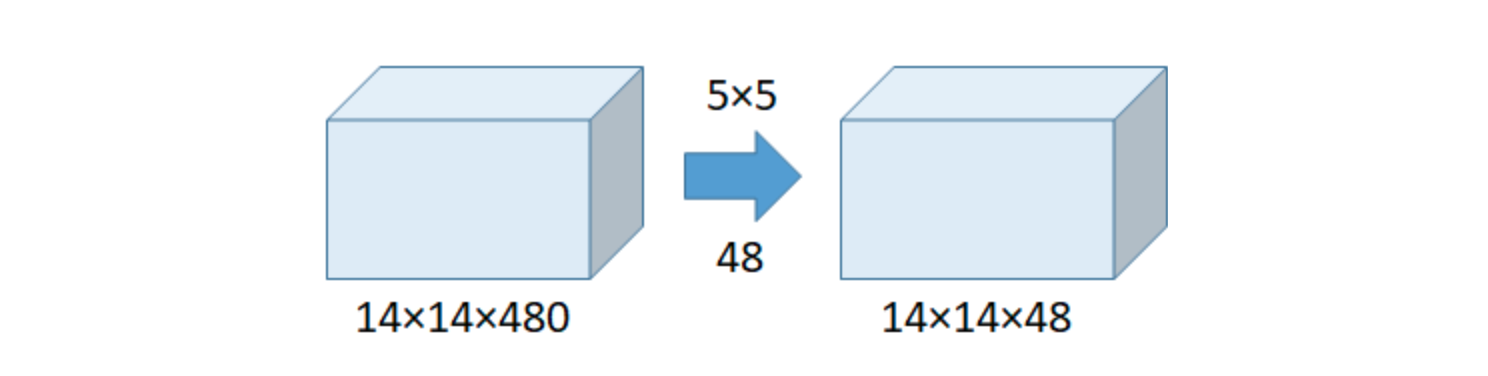
\includegraphics[scale=0.4]{chapter3/InceptionRegularConv}
  \label{fig:InceptionRegularConv}
\end{figure}

Adding a 1 by 1 convolution adds an additional step to the whole transformation but both steps are computationally very efficient. The first step is convolving the input volume with 1 by 1 filters. In our example with 16 filter leading to the following computations: (14x14x16) x (1x1x480) = 3'136 x 480 = 1'505'280. Adding the second 5 by 5 convolution to it leads to (14x14x48) x (5x5x16) = 9'408 x 400 = 3'763'200. Adding the total computations of both convolutions together we get approximately 5.3 million operations compared to 112.9 million computations when not using dimensionality reduction. This is a huge gain in computational efficiency.

\begin{figure}[H]
  \centering
  \caption{First a 1 by 1 convolution is performed in order to reduce the length of the volume leaving the spatial dimensions as is. In the next step a 5 by 5 convolution is performed with 48 filters. \cite{ReviewGoogleLeNetv1}}
  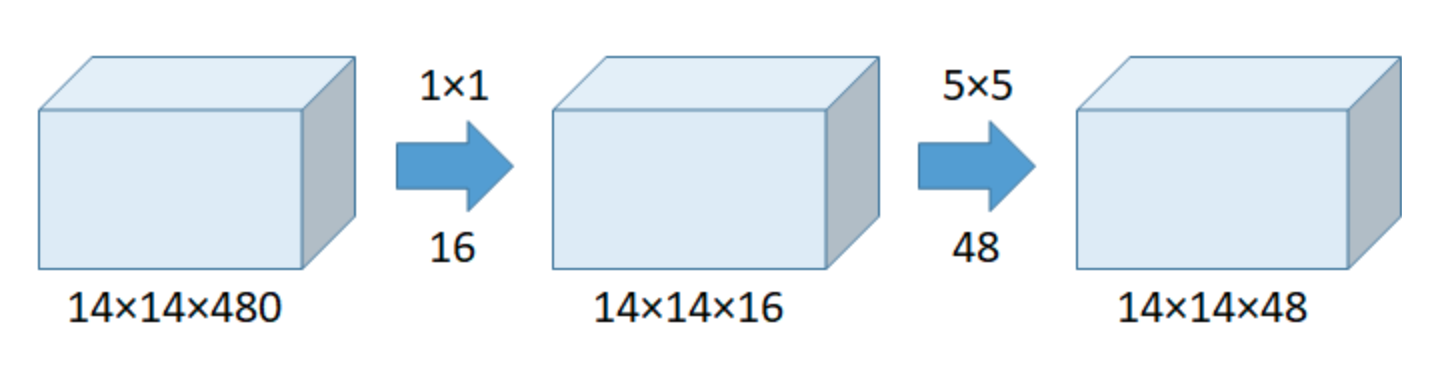
\includegraphics[scale=0.4]{chapter3/InceptionOneByOne}
  \label{fig:parameters}
\end{figure}

This techinque reduces the model size without loosing important information. In contrast, it has been shown, that this technique reduces overfitting and leads to better generalizability.\\

An inception module combines different convolutions together and stacks their output on top of each other. Table \ref{fig:InceptionModuleNaiv} shows a naive inception module without prior dimensionality reduction that would lead to a huge amount of computations needed. 

\begin{figure}[H]
  \centering
  \caption{Naive inception module using different convolution filters and stacking the output on top of each oher. Computationally very expensive. \cite{ReviewGoogleLeNetv1}}
  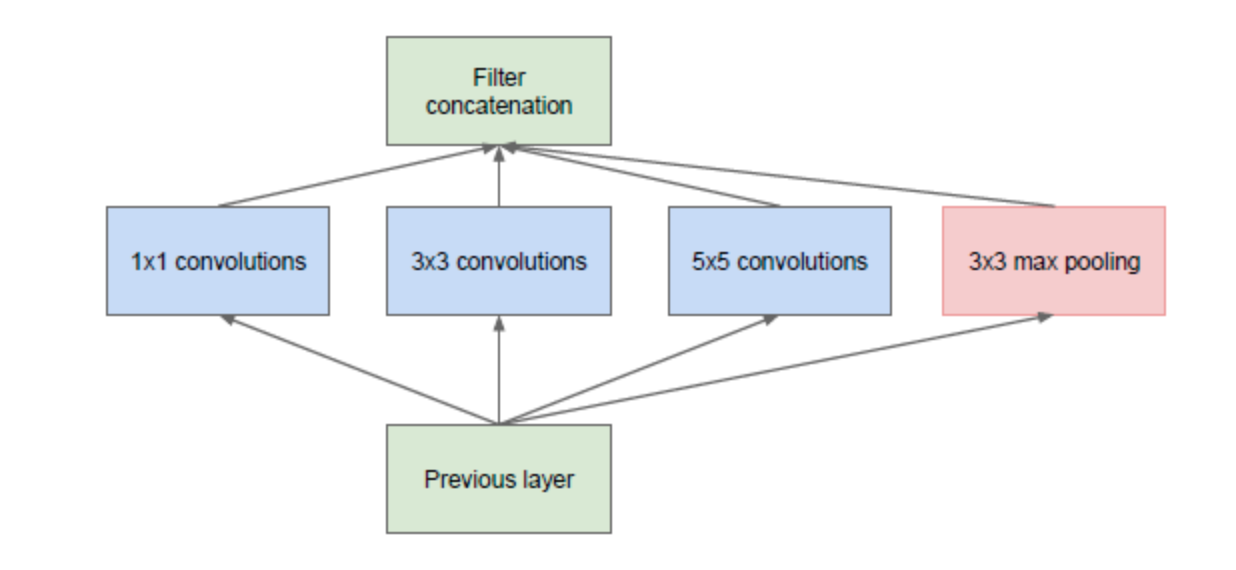
\includegraphics[scale=0.4]{chapter3/InceptionModuleNaiv}
  \label{fig:InceptionModuleNaiv}
\end{figure}

In Table \ref{fig:InceptionModule} the inceptiton module is shown as it is used in the inception network presented in \cite{szegedy2015going} leading to much more efficient implementation. Prior to the different convolutions a 1 by 1 filter is applied on the input volume to reduce the size before the heavy lifting is done. With max-pooling it is the other way around. Max pooling reduces the size without any computational overhead and is therefore performed before the 1 by 1 convolution which requires some amount of compuation.

\begin{figure}[H]
  \centering
  \caption{Inception module with 1 by 1 filters added before doing the different convolutions in order to reduce computation. \cite{ReviewGoogleLeNetv1}}
  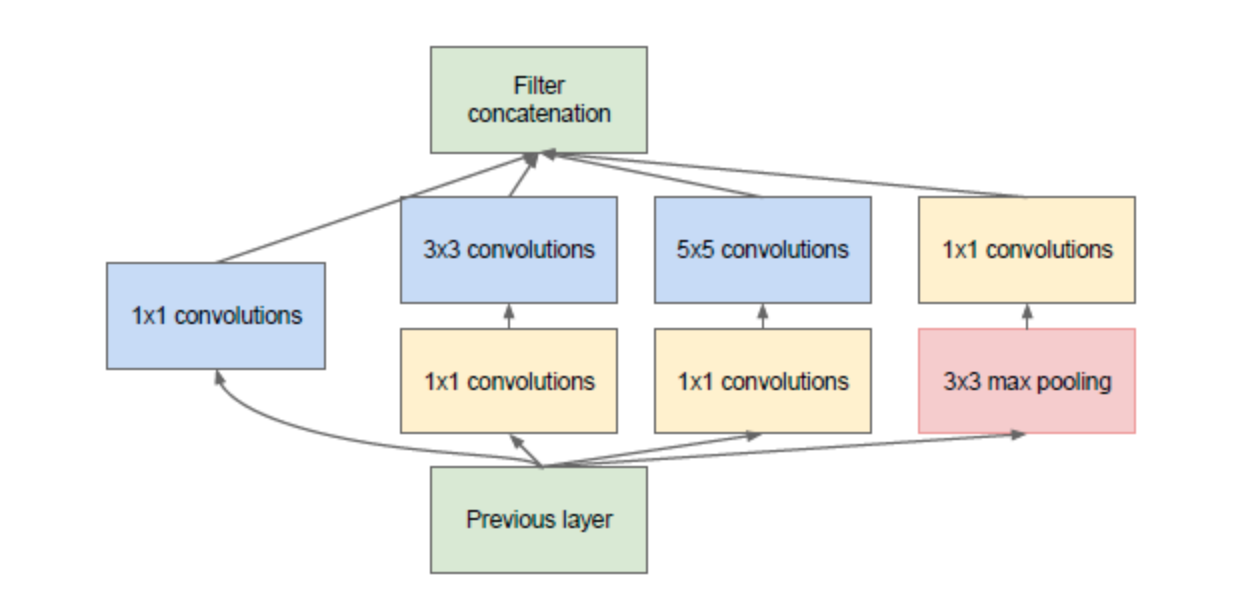
\includegraphics[scale=0.4]{chapter3/InceptionModule}
  \label{fig:InceptionModule}
\end{figure}

The third improvement of GoogLeNet is the global average pooling at the end instead of having three fully-connected layers. AlexNet, ZFNet and VGG all used the common practice to have three fully-connected layers with the last layer being a softmax function. These three last layers made up the bulk of all the parameters used increasing the complexity of the models. Figure \ref{fig:GlobalAveragePooling} shows on the left side a common transition from the a layer with many filter (1024 in that case) to the next layer. 1024 filter with dimension 7 x 7 make 50'176 parameters. If they are fully connected with the next layer which consists of 1024 units it results in 50'176 x 1024 = 51'380'224 weights! With global average pooling as seen on the right side of Figure \ref{fig:GlobalAveragePooling} the 7 x 7 filters get averaged into a 1 x 1 scalar of which 1024 are computed. With averaging the values into one new value no new weights are introduced. Not only is that method much more efficient and reduces the overall complexity but it also can help to reduce the problem of overfitting as mentioned in the Network in Network paper \cite{lin2013network}.

\begin{figure}[H]
  \centering
  \caption{On the left side a commonly used fully connected layer is shown. On the right side a global pooling layer is shown as introduced in GoogLeNet \cite{ReviewGoogleLeNetv1}}
  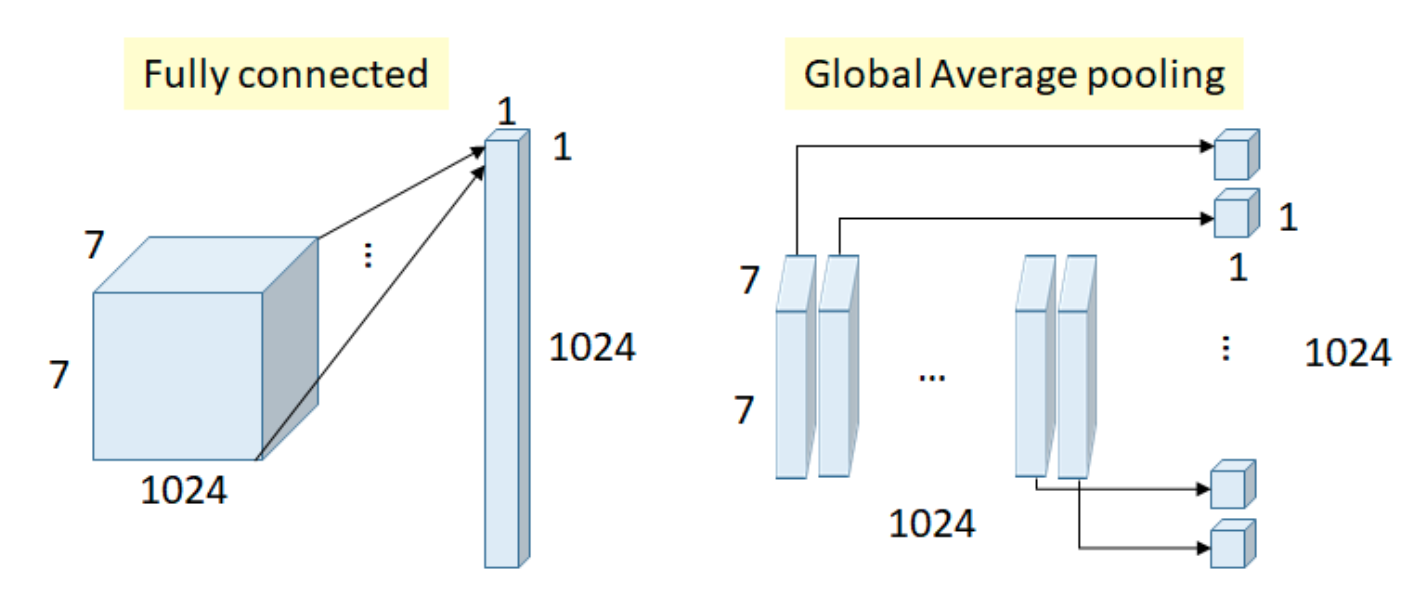
\includegraphics[scale=0.45]{chapter3/GlobalAveragePooling}
  \label{fig:GlobalAveragePooling}
\end{figure}

Inception v3 was the first runner up for image classification in ILSVRC 2015 and came with some refinements over the first version described above \cite{szegedy2016rethinking}. Inception v3 is also used in the Implementation and Evaluation part of this thesis. The first refinment was adding batch normalization \cite{ioffe2015batch}. The second refinement was adding factorizing convolutions to reduce even more parameters without decreasing the architectures efficency leading to the inception v3 model. Table \ref{fig:factorization} shows how a 5 by 5 filter with 25 parameters can be realized with two 3 by 3 filters with 9 parameters each summing up to 18 parameters which is a reduction by 28\%.

\begin{figure}[H]
\centering
\caption{Factorizational Convolution reduces parameters by using smaller filters.}
\subfigure{
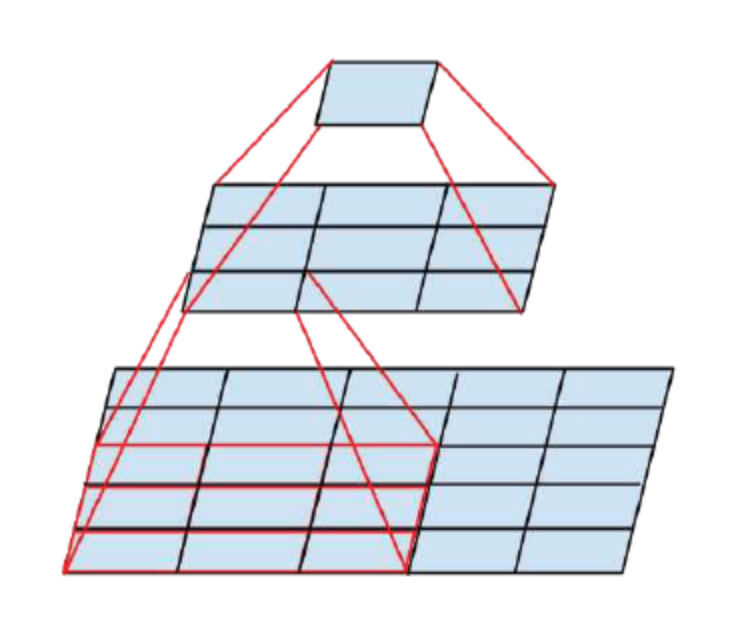
\includegraphics[width=.4\textwidth]{chapter3/FactorizationA}
}
\subfigure{
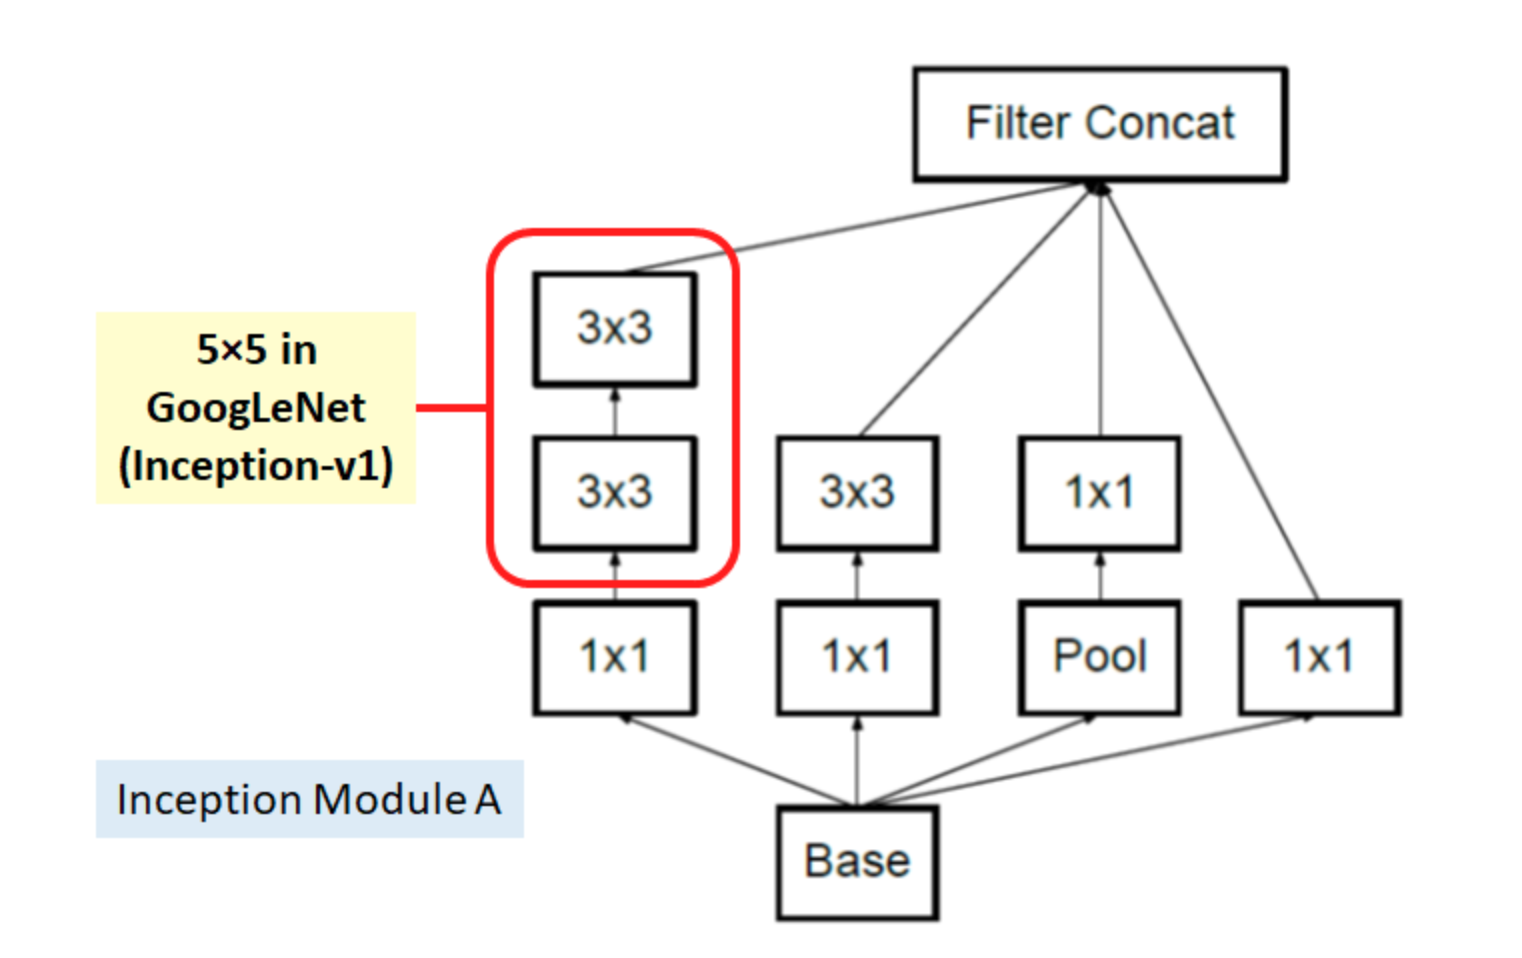
\includegraphics[width=.5\textwidth]{chapter3/FactorizationB}
}
\label{fig:factorization}
\end{figure}

There are additional asymmetric convolutions where a 3 by 3 filter can be realized with two filters of the following sizes: 1 by 3 and 3 by 1. This also reduces the overall parameters used. Another minor modifications are done to the auxiliary classifier and grid size reduction \cite{szegedy2016rethinking}.

\section{ResNet}

The winner of the ILSVRC 2015 were Kaiming He et al. with their very deep architectures applying residual connection connections \cite{he2016deep, he2016identity}. Their architecture was named ResNet and was specifically created with depth in mind. Zeiler et al. have shown how deep networks are naturally able to integrate low/mid/high-level features and that depth seems to enrich these features leading to better performance. Leading results in the ImageNet challenge like the aformentioned VGG \cite{simonyan2014very} and LeNet \cite{szegedy2015going} all exploit deeper architectures. There are a few computational obstacle of going simply deeper with the current models except computational power. One issue arises from the vanishing/exploding gradient which happens during backpropagation \cite{glorot2010understanding}. The weights get updated during learning by multiplying the weights with the gradient from the partial derivatives of the error function. This leads to the chain rule being apllied as many times as layers are present in the network. If the gradient is some small number below 0 it gets multiplied many times over leading to a vanishing value that makes is very difficult to train the layers in the beginning of the network. The same holds true if the gradients are big or above 1. Then they explode by getting bigger and bigger with every layer. But even if the vanishing/exploding gradient can be mitigated with better weight initialization and intermediate normalization layers \cite{ioffe2015batch}, the degradation problem prohibits learning of deeper networks, where the accuracy gets saturated and starts degrading with more layers \cite{he2016deep}. This observed degradation is not caused by overfitting to the training data \cite{he2015convolutional, srivastava2015highway}.\\

ResNet architectures address this degradation problem by introducing residual mappings. These residual mappings are easier to optimize than the unreferenced mapping. If for example it would be optimal to apply the identity mapping, pushing the residual mapping to zero is much easier for the network than fit an identity mapping by a stack of nonlinear layers. Figure \ref{fig:ResidualBlock} shows such a residual block.

\begin{figure}[H]
  \centering
  \caption{A building block for residual learning. \cite{he2016deep}}
  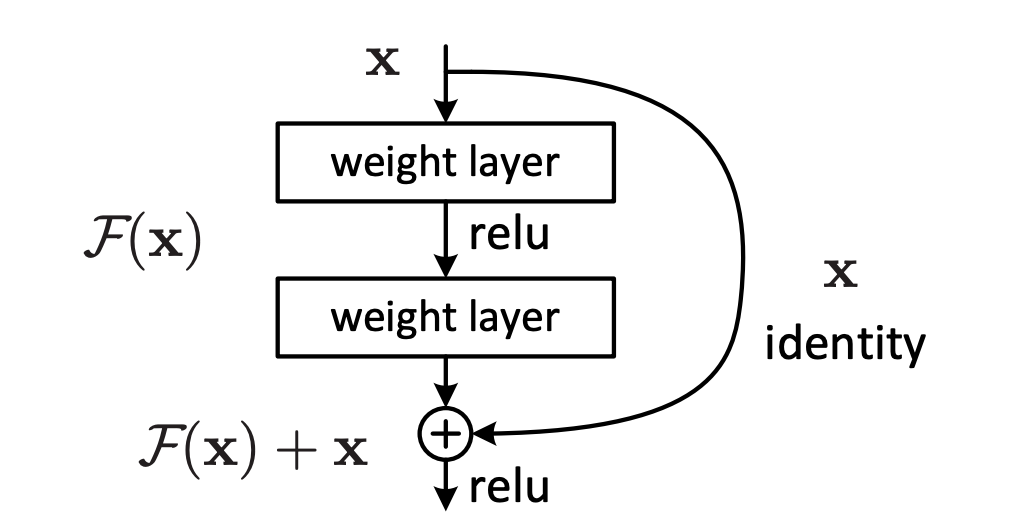
\includegraphics[scale=0.35]{chapter3/ResidualBlock}
  \label{fig:ResidualBlock}
\end{figure}

As seen in Figure \ref{fig:ResNet} blabla blabla

\begin{figure}[H]
  \centering
  \caption{Comparison of the VGG-19 architecture with a 34-layer plain model and its residual counterpart. Notice that only the VGG architecture has 3 fully-connected layers. By omitting these 3 fully-connected layers in the ResNet architecture the overall complexity is drastically reduced. \cite{he2016deep}}
  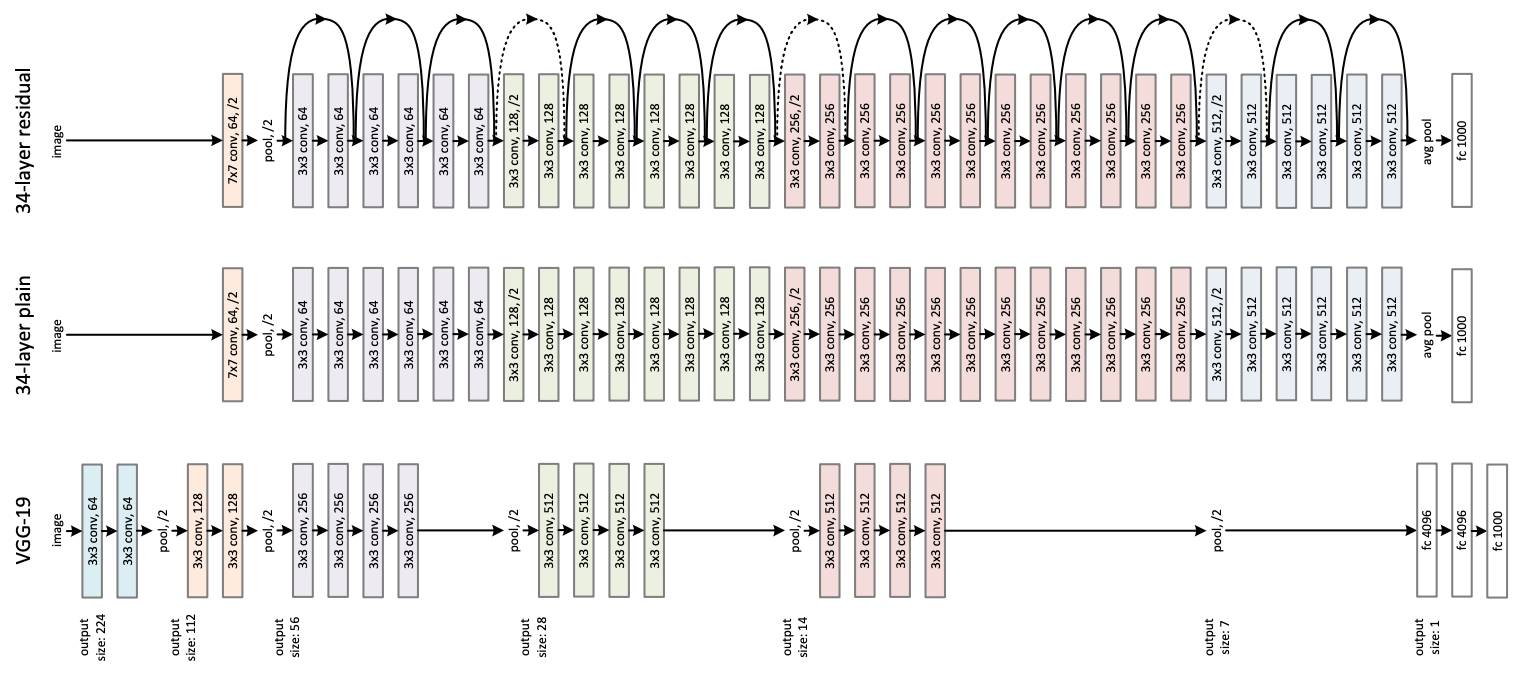
\includegraphics[scale=0.35]{chapter3/ResNet}
  \label{fig:ResNet}
\end{figure}

\section{Densenet}

A common problem of deep networks is the passing of information from layers to layers. A very deep network needs to pass the input through many layers, which can "wash out" by the time it reaches the softmax function or the global average pooling layers. The same holds true for the gradient being passed back to the the beginning of the network. The gradient can vanish or explode as already described with the ResNet architecture. The Dense Convolutional Network (DenseNet) solved this problem with densly connecting all layers with each other that resides in a dense block \cite{huang2017densely}. A dense block
consists of several layers of BatchNormalization, activation function (ReLU) and a SAME convolution that retains the spatial size of the input. Such a dense block is shown in Figure \ref{fig:DenseBlock}. All the layers within the dense block are fully connected with each other in order to implement its own skip connection functionality. The short connections are only possible within a denseblock since all the filters are stacked on top of each other and forwarded to every subsequent layer.

\begin{figure}[H]
  \centering
  \caption{Shown is one dense block of a DenseNet architecture. In the original paper 4 dense blocks were used to create DenseNet. \cite{huang2017densely}}
  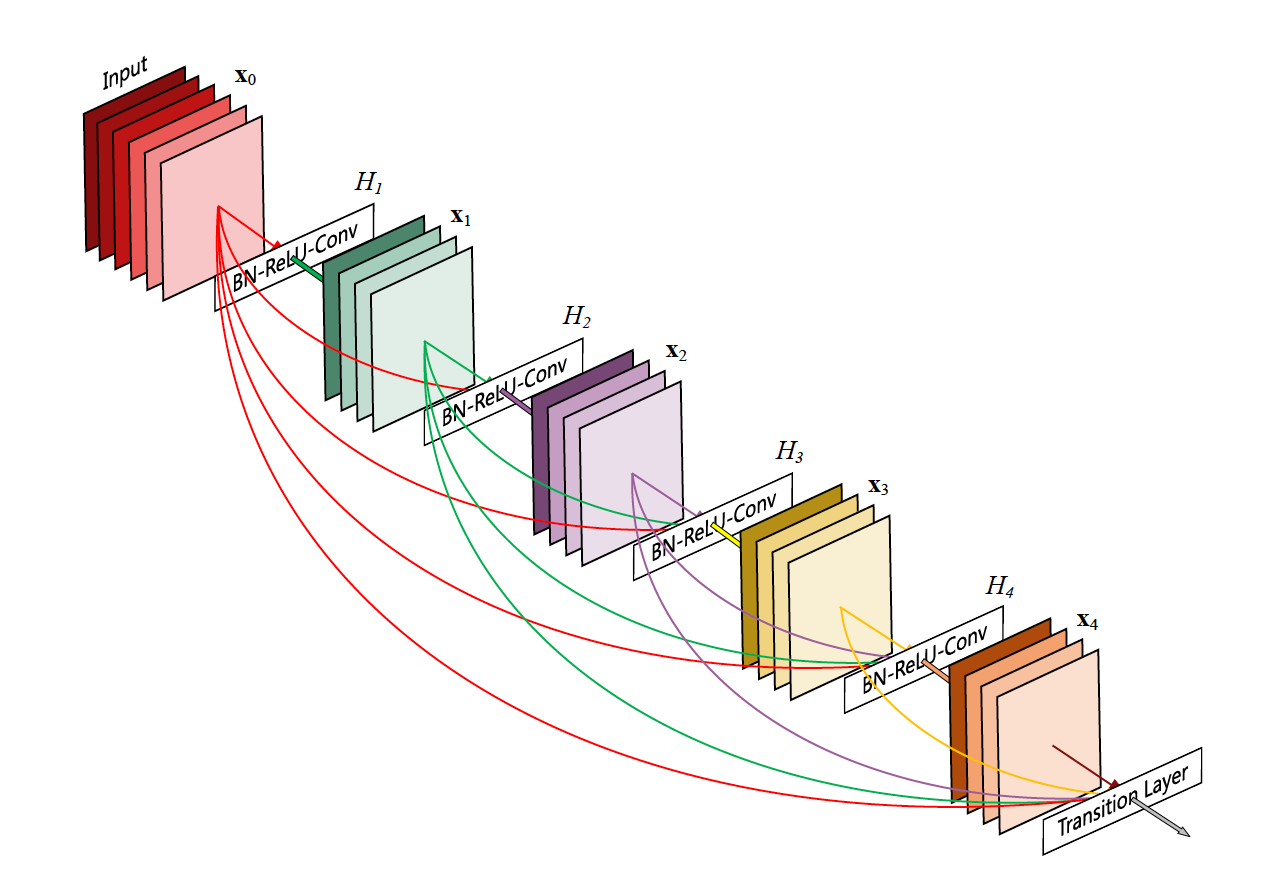
\includegraphics[scale=0.35]{chapter3/DenseBlock}
  \label{fig:DenseBlock}
\end{figure}

After each dense block a 1x1 convolution is used to reduce the number of filters. After this so called bottleneck layer a 2x2 average pooling layer is applied to reduce the spatial dimensions of the input volume as shown in Figure

\begin{figure}[H]
  \centering
  \caption{This Figure shows how the isolated dense blocks are connected through convolution and pooling layers into a full DenseNet architecture. \cite{huang2017densely}}
  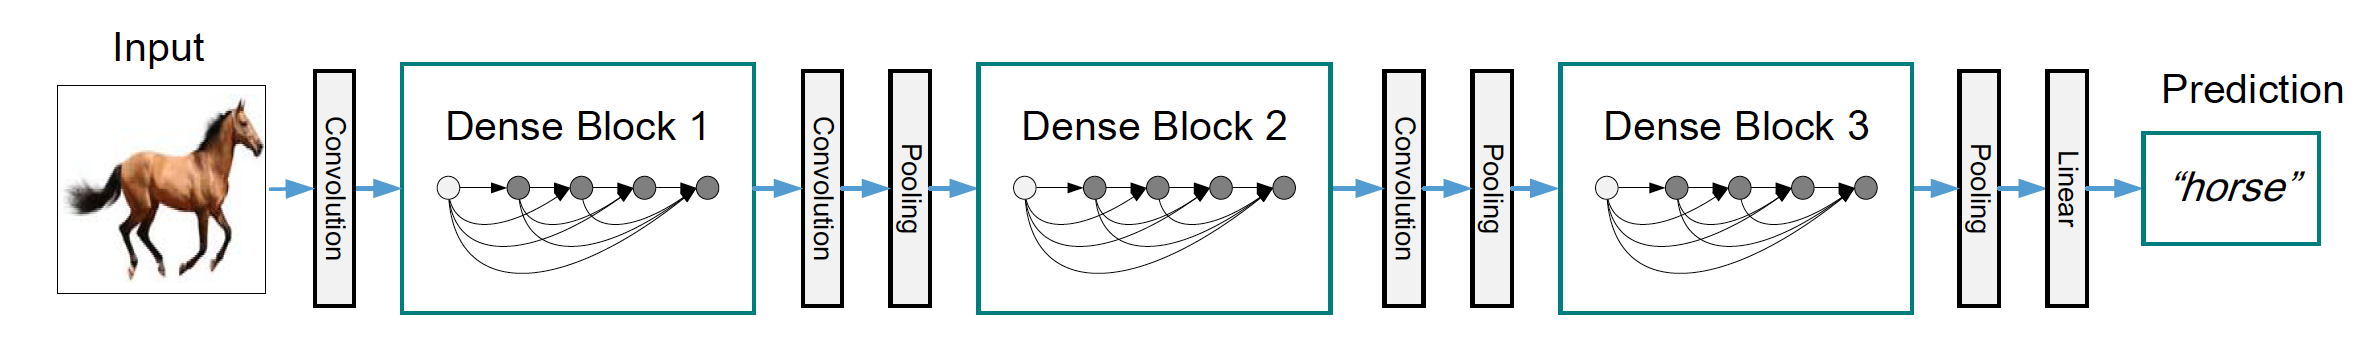
\includegraphics[scale=0.35]{chapter3/DenseNet}
  \label{fig:DenseNet}
\end{figure}

DenseNet introduces several new parameters like the growth rate k which limits the growth of the network and thus limiting the width of the network. A growth rate of 12 means that each layer may only add another 12 filters to the existing filters prior to this layer. Another interesting parameter is the compression which improves the compactness of the model by defining how much of the feature-maps get transitioned to the next dense block. The compression value is between 0 and 1 without including the value 0.